\begin{figure}[h!]
\centering
\psfrag{mg}[cc][cc][1][0]{\scriptsize$m\textbf{g}$}
\psfrag{Me}[cc][cc][1][0]{\scriptsize$M_e$}
\psfrag{te}[cc][cc][1][0]{\scriptsize$\mathbf{f}_e$}
\psfrag{f1}[cc][cc][1][0]{\scriptsize$-f_2\textbf{e}_2$}
\psfrag{f2}[cc][cc][1][0]{\scriptsize$-f_1\textbf{e}_1$}
\psfrag{f3}[cc][cc][1][0]{\scriptsize$-f_3\textbf{e}_2$}
\resizebox{0.5\textwidth}{!}{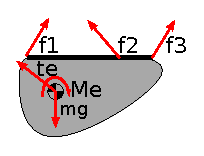
\includegraphics{img/equilibre_stat_ext.eps}}
\caption[DCL de l'effecteur avec forces externes]{\label{chap1:fig:equi_stat_ext}Diagramme de corps libre de l'effecteur lors de l'application d'un torseur d'action mécanique $\mathbfcal{T}=[\mathbf{f}_e,M_e]^T$ .}
\end{figure}